\chapter{TECNOLOGIAS}
\label{cha: Conceituacaoo e Ideia Geral}

Nas seções a seguir explicaremos os principais conceitos que utilizaremos para o desenvolvimento do nosso trabalho, as ferramentas utilizadas, fontes de dados exploradas e tecnologias aproveitadas para melhorar o entendimento do tema de nosso trabalho. 

A seção \ref{sec: Redes sociais} descreve as principais redes sociais que podem ser usadas em nossa aplicação, e a seção \ref{sec: API} relata o uso de suas APIs.
A seção \ref{sec: analiseSentimento} contextualiza um dos possíveis usos futuros de nossa aplicação.
Em \ref{sec: Cloud9} é apresentado o ambiente de desenvolvimento em nuvem que utilizamos durante o desenvolvimento da aplicação.
Já a seção \ref{sec: Framework} define o termo Framework, a \ref{sec: MVC} apresenta o padrão de projeto que usaremos, e na seguinte, \ref{sec: Ruby} explica o básico da linguagem de programação que escolhemos para nossa aplicação.
A seção \ref{sec: Rails}, mostra o framework escolhido para o desenvolvimento do trabalho. 
Na seção \ref{sec: BDRelacional} apresentaremos o conceito de banco de dados. % SGBD: colocar no dic. de siglas.
% e, em suas subseções, \ref{subsec: BDRelacional} e \ref{subsec: ActiveRecord} são explicados o conceito de um banco de dados relacional e a biblioteca responsável pelo gerenciamento dos dados, respectivamente.
% e em suas subseções \ref{subsec: FacebookAPI}, \ref{subsec: RedditAPI}, \ref{subsec: YoutubeAPI} e \ref{subsec: TwitterAPI}, serão explicadas as APIs do Facebook, Reddit, Youtube e Twitter, respectivamente.  % mudar esquema das subsecoes

\section{Redes sociais}
\label{sec: Redes sociais}
Rede social é um site dedicado ou um aplicativo que permite que os usuários se comuniquem uns com os outros por meio da publicação de informação, comentários, mensagens, imagens, vídeos ou outros recursos \cite{socialNetworkDefinition}.

Com a popularização da internet, surgiram vários sites que possuem essa estrutura, alguns deles já não existem mais, como o Orkut, já outros recebem muitos acessos ainda hoje como Facebook, Twitter, Youtube, Google+, MySpace, LinkedIn, Reddit, Instagram e Tumblr \cite{wsj}.

Para se ter uma ideia da proporção de pessoas que acessam essas estruturas sociais, considere se o número de usúarios do Facebook fosse a população de um país, ele se tornaria o país mais populoso do mundo \cite{facebookPais}.
Nessa seção apresentaremos uma visão sobre as redes sociais que fazem parte da base do nosso trabalho:  seção \ref{subsec: Facebook} Facebook, seção \ref{subsec: Reddit} Reddit, seção \ref {subsec: Twitter} Twitter, e na seção \ref{subsec: Youtube}  Youtube. Os textos contidos neles possuem conteúdo de caráter opinativo, o que é favorável para aplicações de análise de sentimento.

    \subsection{Facebook}
    \label{subsec: Facebook}
É uma rede social que visa conectar as pessoas aos seus familiares e amigos \cite{FBnewsroom}, permitindo que o usuário crie um perfil, publique textos, fotos, vídeos, envie mensagens e mantenha contato com quem deseja. Foi criada em 2004 por estudantes da Universidade de Harvard e hoje é a maior rede social do mundo, com mais de 1 bilhão de usuários \cite{Facebook101}.

    \subsection{Reddit}
    \label{subsec: Reddit}
É uma comunidade online de mídia social que permite que seus usuários votem e comentem nos conteúdos postados. Podem ser criadas sub-comunidades, chamadas sub-reddits, cujos conteúdos são independentes do Reddit, normalmente com um assunto em comum e moderadas por um grupo de voluntários \cite{WhatIsReddit}. \par
O Reddit é uma fonte de novidades e assuntos populares na internet. Seus usuários produzem o conteúdo e votam em conteúdos postados por outros. Os que recebem grandes quantidades de votos positivos da comunidade, tendem a aparecer no topo da página, sendo assim a página principal mostrará conteúdos novos e relevantes para os leitores \cite{RedditWiki}.
    
    \subsection{Twitter}
    \label{subsec: Twitter}
O Twitter é uma rede social que permite que seus usuários enviem e leiam mensagens curtas de no máximo 140 caracteres chamadas “tweets”.

Atualmente, o Twitter está entre os 10 sites mais acessados do mundo \cite{twitterOverview}, com 288 milhões de usuários ativos por mês e 500 milhões de tweets por dia \cite{aboutTwitter}.

Muitos usuários desse serviço o usam para postar sua opinião sobre outros serviços ou produtos, seja ela uma reclamação ou um elogio, e isso torna essa rede uma importante fonte de dados para nossa aplicação \cite{PAK10.385}.

    \subsection{Youtube}
    \label{subsec: Youtube}
O Youtube foi fundando em maio de 2005 com a finalidade de proporcionar a seus usuários a pesquisa, o entretenimento e o compartilhamento de vídeos em formato digital \cite{SobreYoutube}.

Esse sítio também é considerado uma rede social, pois possui as seguintes características \cite{Benevenuto}:
\begin{enumerate}
    \item Permite construir um perfil publico, ou semipúblico;
    \item Proporciona ao usuário uma lista de outros usuários com os quais ele(a) pode compartilhar informações;
    \item Possibilidade de visualizar e percorrer suas listas de conexões ou as listas criadas por outros usuários.
\end{enumerate} 

O que torna essa rede social relevante para este trabalho é a possibilidade de usuários comentarem em vídeos armazenados por outros usuários da rede, assim expondo sua opinião, seja ela positiva ou negativa, sobre o tema abordado no vídeo.

Os comentários são o principal meio de comunicação entre os usuários do Youtube, e isso os torna uma fonte importante para extração de dados.
Os usuários podem indicar se gostaram de uma publicação específica através do botão \textit{like}, ou se não gostaram através do botão \textit{dislike}. Isto possibilita avaliar quais publicações são mais populares e as menos. Estas características o tornaram um bom candidato para executar a nossa aplicação.

\section{API}
\label{sec: API}

Chamamos de API (Application Programming Interface) um conjunto de comandos, protocolos e funções estabelecidos por um software, com a finalidade de acessar suas funcionalidades sem precisar conhecer seus detalhes de implementação \cite{APIDef}.

Utilizaremos \textbf{APIs web}, que geralmente usam requisições HTTP\footnote{Protocolo usado na transferência de dados pela internet \cite{HTTPDef}.} para enviar mensagens a servidores específicos, que por sua vez retornam uma resposta HTTP geralmente nos formatos XML\footnote{XML é usado para descrever documentos em um formato padrão que pode ser lido por qualquer aplicação compatível com XML \cite{XMLDef}.} ou JSON\footnote{JSON é um formato para trocas de dados estruturados baseados em texto. JSON é comumente usado como uma alternativa ao XML, pois sua forma de representar os dados é mais compacta \cite{JSONDef}.}, com o conteúdo referente à requisição feita.
Toda requisição feita a uma API web precisa de autorização. Para isso a maioria das APIs web utilizam um protocolo chamado OAuth 2.0, que funciona sobre o HTTP e gerencia as autorizações através de uma chave de acesso chamada \textit{access token}.

Na seção acima apresentamos os principais usos das redes sociais Facebook, Reddit, Twitter e Youtube. Como cada uma possui um foco diferente, é natural que cada API aborde da melhor forma seu contexto predominante.

Abaixo iremos explicar as especificidades de cada uma das APIs que usaremos neste trabalho.

% \begin{figure}[ht]
%   \centering
%   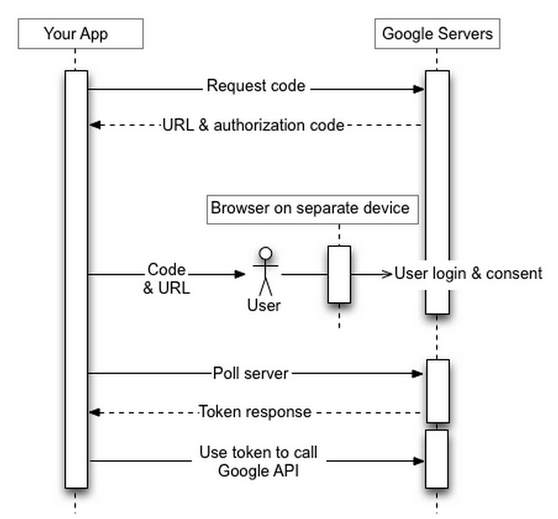
\includegraphics[width=.8\textwidth]{images/accessToken}
 
%   \caption{Procedimento da conta de serviço obtendo o token de acesso \cite{JSONDef}.}
%   \label{fig:accessToken}
% \end{figure}

% Vamos tomar como exemplo o funcionamento de uma requisição à API do Google. As credenciais de uma conta de serviço, que se obtém do Google Developers Console, inclui um endereço de e-mail gerado, que é único, um ID do cliente, e pelo menos um par de chaves: pública e privada. Usa-se o ID do cliente e a chave privada para criar um JWT\footnote{JSON Web Token (JWT) é uma forma compacta de representar reivindicações a serem transferidas entre duas partes. Essas reivindicações em um JWT são codificadas em um objeto no formato JSON e criptografadas ou assinadas digitalmente \cite{APIDef}.} assinado e construir uma solicitação de token de acesso no formato adequado. O seu aplicativo envia a solicitação para o Google OAuth Server 2.0, que retorna um token de acesso. O aplicativo usa o token para acessar uma API do Google. Quando o token expira, repete-se o processo \cite{JSONDef}.

    \subsection{Facebook API}
    \label{subsec: FacebookAPI}
Outra API que possibilitaria uma excelente extração de dados para o nosso sistema é a do Facebook, pois além da pesquisa de publicações públicas, poderíamos também usar as curtidas em fanpages de cada pessoa, para filtrar opiniões de usuários que demonstrem interesse no assunto procurado.

Nós conseguimos utilizar a API do Facebook, entretanto sua atualização para a versão 2.0 e as seguintes conta com uma grande alteração nas permissões que um aplicativo pode utilizar, duas delas impactam diretamente no nosso:
\begin{itemize}
  \item Indisponibilizada a pesquisa de objetos públicos, como as publicações que pretendíamos utilizar \cite{FacebookDevs}.
  \item Indisponibilizado o acesso à lista de amigos de um usuário que não usa seu aplicativo \cite{FacebookDevs}.
\end{itemize}

Estas permissões foram retiradas porque algumas pessoas se sentiam desconfortáveis ao ter suas informações sendo acessadas sem sua permissão direta, como explicado no vídeo oficial do canal Facebook Developers \cite{FbAPIV2Video}.
Como nosso aplicativo depende que as APIs forneçam acesso aos dados públicos dos usuários e o Facebook revogou-os nas versões 2.0 e posteriores da API, tivemos que descartá-lo como fonte de dados.

    \subsection{Reddit API}
    \label{subsec: RedditAPI}
O reddit disponibiliza uma série de informações por sua API, em formato JSON, disponíveis por requisições HTTP simples \cite{RedditAPIWordpress}.
Os recursos\footnote{Um recurso é um conjunto de dados que representa um determinado objeto.} que utilizaremos para construção da nossa aplicação são:
\begin{itemize}
    \item Listing - Uma lista de links.
    \item Comment - Um objeto que representa um comentário em um link.
    \item Client - Um objeto “cliente”, no nosso caso usaremos um usuário e senha em branco, para que criemos um cliente anônimo.
\end{itemize}
Os demais recursos podem ser encontrados no anexo \ref{fig: RecursosReddit}.
Cada recurso permite o uso de um conjunto de operações, por exemplo, um recurso Client, pode executar a operação \textit{search} que irá retornar uma \textit{Listing} (lista de links) que contém os termos passados como parâmetro para a operação \cite{RedditAPISearch}.

Outra operação muito útil para nossa aplicação é a Comments. Executada por um recurso Client, essa operação retorna uma árvore de comentários do link passado por parâmetro, comentários esses que também servirão como textos a serem armazenados pela nossa aplicação.
%[5]
    
    \subsection{Twitter API}
    \label{subsec: TwitterAPI}
A API do Twitter provê acesso à leitura e escrita de dados no Twitter através de requisições HTTP, que podem ser invocadas por códigos escritos em alguma linguagem de programação. Hoje, a versão mais recente da API do Twitter é a 1.1 \cite{TwitterRestApi}.

Algumas possíveis ações são: criar um novo tweet, ler o perfil de um usuário da rede e buscar tweets públicos que possuem um termo em comum \cite{TwitterRestApi}.

Requisições HTTP feitas usando a API do Twitter possuem parâmetros, sendo alguns necessários e outros opcionais. Por exemplo, para buscarmos tweets através de um termo específico devemos especificar o termo em questão como um parâmetro \cite{TwitterSearchApi}.

A URL\footnote{URL, do inglês "Uniform Resource Locator" é o endereço de um site específico da Web ou de um arquivo na Internet \cite{URLDef}.} de uma requisição HTTP a API do twitter versão 1.1 possui o seguinte formato: https://api.twitter.com/1.1/recurso?parametros, substituindo “recurso” e “parâmetros” conforme as necessidades aplicação.

    \subsection{Youtube API}
    \label{subsec: YoutubeAPI}
A API de dados do YouTube (versão 3) permite buscar resultados de pesquisa e recuperar, inserir, atualizar e excluir recursos, como vídeos ou playlists \cite{YouTubeAPI}.

Para criar uma aplicação utilizando a API do Youtube, é necessário criar uma conta no Google para acessar o Console de APIs do Google, solicitar uma chave da API e cadastrar seu aplicativo (caso queira cadastrar um aplicativo veja o apêndice \ref{sec: CadastrandoApp}) \cite{GettingStartedYoutubeAPI}. Com a aplicação cadastrada, temos acesso aos recursos da API. Alguns tipos de recursos da API do Youtube são \cite{GettingStartedYoutubeAPI}:

\begin{itemize}
  \item channel: Contém informações sobre um canal\footnote{ Página principal de uma conta no Youtube.} simples do YouTube.
  \item guideCategory: Identifica uma categoria que o YouTube associa aos canais com base em seu conteúdo ou outros indicadores, como a popularidade.
  \item search result: Contém informações sobre um vídeo, um canal ou uma playlist do YouTube que corresponde aos parâmetros de pesquisa especificados em uma solicitação da API.
\end{itemize}

Outros exemplos de recursos serão encontrados na tabela \ref{fig: RecursosYoutube} nos apêndices \ref{cha: apendices}.

Alguns recursos são compatíveis com operações que executam funções mais específicas a esses recursos. Por exemplo, o recurso search result tem uma operação que recupera uma lista, no qual pode estar vazia ou conter vários recursos \cite{GettingStartedYoutubeAPI}.

Existem operações que precisam de autorização para usar um recurso. Mas existem outras, como a list que não precisam de autorização para serem usadas. 

Nos anexos, pode-se encontrar a tabela \ref{fig: OperacoesCompativeis} que lista as outras operações da API, e a tabela \ref{fig: OperacoesCompativeisComRecursos} que exibe as operações que são compatíveis com cada recurso.

Cada operação tem um custo, que é determinado pela quantidade de memória, CPU e de recursos de rede. Então para garantir que os desenvolvedores usem o serviço de uma forma justa, o Google impõe uma quota, que é um limite de operações que a aplicação pode fazer em um determinado intervalo de tempo \cite{GettingStartedYoutubeAPI}.

Para evitar a transferência, a análise e o armazenamento de dados desnecessários, a API permite a recuperação de recursos parciais. Para isso, esta é compatível com dois parâmetros de solicitação, que permitem identificar as propriedades de recursos que devem ser incluídas nas respostas da API.

\begin{itemize}
	\item O parâmetro part identifica grupos de propriedades que devem ser devolvidas a um recurso. 
	\item O parâmetro fields filtra a resposta da API para devolver apenas propriedades específicas nas partes de recurso solicitadas.
\end{itemize}

\section{Análise de sentimento}
\label{sec: analiseSentimento}
A Análise de sentimento é um campo de estudo que analisa as opiniões, sentimentos, avaliações, atitudes e emoções expressadas por pessoas por meio de textos\cite{ASOpinionMining}.
Desde 2000, vem crescendo para ser uma das áreas de pesquisa mais ativas no processamento de linguagens naturais \cite{ASOpinionMining}. Difundiu-se de ciência da computação para ciências empresariais e ciências sociais, devido a sua importância aos negócios e sociedade como um todo \cite{ASOpinionMining}.

A importância crescente da análise de sentimento coincide com o crescimento da mídia social, tais como comentários, fóruns de discussão, blogs, micro-blogs, Twitter e redes sociais \cite{ASOpinionMining}. Pela primeira vez na história humana, temos agora um enorme volume de dados opinativos gravados em formato digital para análise \cite{ASOpinionMining}.

A análise de sentimento aborda várias áreas de pesquisa. No presente trabalho, utilizaremos a medição de quão negativa ou positiva são as opiniões de um grupo de indivíduos \cite{ASFerreiraEBA}. Os dados de entrada para a análise de sentimento são aqueles tornados públicos em redes sociais.

Utilizando a análise de sentimento, esses dados podem passar de simples textos dentro de um banco de dados, para estatísticas sobre a opinião de um conjunto de pessoas acerca de determinados assuntos.

\section{Cloud9}
\label{sec: Cloud9}
A Cloud9 é um ambiente de desenvolvimento (IDE) que visa melhorar a codificação e atender as necessidades atuais dos desenvolvedores. Um serviço baseado em Computação em nuvens\footnote{A computação em nuvem é um conceito de utilizar a memória, a capacidade de armazenamento, e os recursos de um servidor compartilhando-os por meio da Internet \cite{ComputacaoNuvem}.}, rodando diretamente do navegador, sem necessidade de instalação de nenhum aplicativo adicional, permitindo também executar, depurar, e criar aplicativos de qualquer lugar, a qualquer hora e com outras pessoas simultaneamente \cite{C9ComoUsar}.

\section{Framework}
\label{sec: Framework}
Em geral, um Framework é uma estrutura básica para alguma coisa específica \cite{FrameworkByMerriam}. Portanto, no contexto de desenvolvimento de software, um Framework é uma base para que desenvolvedores de software possam construir programas para uma plataforma específica \cite{FrameworkDef}.

Existem muitos frameworks diferentes para desenvolvimento de aplicações web, cada um com suas utilidades e funcionalidades. Utilizar um framework apropriado no desenvolvimento de uma aplicação pode economizar uma grande quantidade de tempo, além de manter o código organizado e padronizado, o que gera maior facilidade na manutenção do mesmo \cite{FrameworkDocForge}.

\section{Model-view-controller}
\label{sec: MVC}

A arquitetura \textit{Model-View-Controller} (Modelo-Visão-Controlador) tem como objetivo principal fazer uma ponte entre o modelo mental do usuário humano e o modelo digital que existe no computador \cite{Trygve/MVC}.
Sua infraestrutura é dividida em 3 partes \cite{MVC}:

\begin{itemize}
    \item Modelo (model): Contém todo o conteúdo, lógica de processamento e funções, afim de separar os dados.
    \item Visão (view): pode ser qualquer saída de representação dos dados, como uma tabela ou um diagrama, ou seja, como o nome já diz é a visão externa requerida pelo usuário final.
    \item Controlador (controller): faz a mediação entre os acessos ao modelo e à visão e coordena o fluxo de dados entre eles.
\end{itemize}

Inicialmente construída para solucionar problema em geral de usuários que controlam um conjunto de dados grandes e complexos. No entanto o MVC foi adaptado como uma arquitetura para as aplicações Web \cite{WikipediaMVC}.

Foram criados muitos frameworks (seção \ref{sec: Framework}) de aplicação com base nesse modelo, variando em suas interpretações, principalmente no modo que as responsabilidades MVC são divididas entre o cliente e servidor \cite{WikipediaMVC}.

Os frameworks web MVC mais recentes foram adaptados para um modelo cuja visão e a lógica do controlador estão dentro de um servidor \cite{WikipediaMVC}.

Como a complexidade das aplicações sempre visa a programação orientada a objeto, a separação entre dados e a apresentação das aplicações acaba sendo relevante, logo esse padrão atende a esse problema através da separação das tarefas de acesso aos dados e a lógica \cite{WikipediaMVC}.

\section{Ruby}
\label{sec: Ruby}
Ruby é uma linguagem de programação orientada a objeto\footnote{Programação orientada a objetos é uma tentativa de representar os “objetos” que encontramos no mundo real em um software \cite{ObjectOrientedProgramming}.} criada por Yukihiro Matsumoto.

Assim como Perl\footnote{Pearl: Uma linguagem de programação de alto nível e propósito geral usada especialmente para desenvolvimento de aplicações Web \cite{PerlDef}.}, Ruby é apropriada para processamento de textos, pois além de tratar tudo como um objeto, possui blocos e iteradores especiais que facilitam o manuseio de textos \cite{RubyFAQ}.

Nesse trabalho usaremos Ruby aliado ao framework Ruby on Rails, pois essa linguagem apresenta as funcionalidades necessárias para resolver, de forma eficiente, os problemas que encontramos no desenvolvimento dessa aplicação.

    \subsection{Gemas}
    \label{subsec: Gemas}
Assim como a maioria das linguagens de programação, Ruby também possui bibliotecas de funções. A maioria dessas bibliotecas estão na forma de gemas \cite{RubyLibs}. Dentro de uma gema estão os seguintes componentes:
% respondendo o questinamento do bruno, sobre outros formatos de biblitoecas. Acessando a referência:
% "Most of them are released in the form of a gem. [...] Some other libraries are released as archived (.zip or .tar.gz) directories of source code."

\begin{itemize}
    \item Código (Incluindo códigos para testes e outras utilidades)
    \item Documentação
    \item gemspec
\end{itemize}

O arquivo gemspec contém informações importantes sobre a gema como nome, versão e autores \cite{WhatIsGem}.

Para instalar uma gema, usa-se o gerenciador de pacotes RubyGems, que facilita a criação, o compartilhamento e a instalação dessas bibliotecas \cite{RubyLibs}.

\section{Ruby on Rails}
\label{sec: Rails}
Ruby on Rails é um framework de desenvolvimento web de código aberto e que utiliza a linguagem de programação Ruby \cite{RubyOnRails}. Ele contém o que é necessário para desenvolver aplicações web\footnote{Uma aplicação web é um programa cujo processamento de informações é realizado do lado do servidor e o resultado do processamento é enviado, quando permitido, para o cliente que as requisitou via um navegador de internet \cite{TechTerms}.}, com suporte a banco de dados, de acordo com o padrão de projeto de software Model-View-Controller (MVC) \cite{APIRails}.

    \subsection{Motivação}
    \label{subsec: Motivos Rails}
Tendo em vista que as fontes para nosso software são aplicações web, decidimos optar por desenvolver o nosso programa também como uma aplicação web. Utilizaremos o framework Ruby on Rails por já termos estudado-o anteriormente, possuirmos certa afinidade com a linguagem, rapidez de desenvolvimento que ele proporciona e também por existir ótima documentação para o uso das APIs que precisaremos.

Outro ponto que nos fez optar pelo Ruby on Rails foi a agilidade e facilidade que ele oferece para adaptar a modelagem e informações de bancos de dados, que é um de seus pontos fortes como framework de desenvolvimento web \cite{AtlasWeb}.
    
\section{Banco de dados relacional}
\label{sec: BDRelacional}

Um banco de dados relacional é uma coleção de dados organizados em conjuntos de tabelas descritas formalmente, que permite que os dados possam ser acessados, ou manipulados, de maneiras diferentes sem precisar reorganizar as tabelas de banco de dados \cite{RelDatabase}.
Se um banco de dados suporta o modelo relacional, ele organiza seus dados em relações, que por sua vez podem ser vistas como tabelas. Cada coluna de uma tabela representa um atributo da relação, e as linhas representam aos registros \cite{BancoRelacional}.

Um conceito fundamental em um banco de dados relacional é o conceito de atributo chave, que permite identificar e diferenciar um registro de outro. Utilizando atributos chave é possível estabelecer relacionamentos entre duas ou mais tabelas, além de tornar mais rápido o acesso a elementos, usando índices \cite{BancoRelacional}.
Dois dos fatores que contribuem com o sucesso do modelo relacional em bancos de dados é o forte embasamento matemático \cite{FundamentosBD} na definição dos conceitos utilizados e a uniformização da linguagem de manipulação de banco de dados(SQL) \cite{BancoRelacional}.

\subsection{Sistema de gerenciamento de banco de dados}
\label{subsec: SGBD}

Um sistema de gerenciamento de banco de dados (\gls{SGBD}) é um conjunto de programas de software que permite que usuários criem, editem, atualizem, armazenem e recuperem dados em banco de dados de forma mais prática e segura \cite{SGBD}. 

    \subsection{PostgreSQL}
    \label{subsec: PostgreSQL}
	
O PostgreSQL é um \gls{SGBD} de código aberto com mais de 15 anos de desenvolvimento ativo \cite{SobrePostgreSQL}. Considerado o \gls{SGBD} de código aberto mais seguro e avançado \cite{OverviewPostgreSQL}.
Ele, assim como a maioria dos \gls{SGBD}\textbf{s}, segue o padrão de linguagem SQL\footnote{SQL - Structured Query Language é uma linguagem de consulta e manipulação de bancos de dados.} ANSI\footnote{ANSI - American National Standards Institute} e possui extensões próprias para sua linguagem SQL \cite{SQLIntro}.

    \subsection{Active record}
    \label{subsec: ActiveRecord}

Active Record é a gema utilizada pelo framework Ruby on Rails que representa a camada de modelo da aplicação. Esta camada é responsável pelo Mapeamento objeto-relacional\footnote{Mapeamento objeto-relacional - Técnica de desenvolvimento utilizada para reduzir o trabalho necessário de adaptação de um software programado, usando orientação a objeto para utilizar um bancos de dados relacional. As tabelas do banco de dados são representadas na aplicação como classes, e os registros de cada tabela são representados como instâncias das classes correspondentes \cite{ORM}.}, facilitando a criação e o uso dos objetos da aplicação cujos dados precisam de armazenamento persistente\footnote{Armazenamento persistente: Forma de armazenar dados para continuarem a existir mesmo após o término do programa que os criou \cite{BDOO}.} \cite{ActiveRecordBasics}.

Os objetos Active Record não tem seus atributos definidos diretamente, mas sim, inferidos da definição da tabela que representa sua classe. Caso atributos ou tipos desse objeto sejam adicionados, alterados ou removidos, a mudança será realizada também na base de dados, diretamente \cite{ActiveRecordDocs}.